\documentclass[10pt]{beamer}
\usefonttheme{professionalfonts} % using non standard fonts for beamer
\usefonttheme{serif} % default family is serif
\usepackage[utf8]{inputenc}
\usepackage[export]{adjustbox}
\usepackage{tikz}
\usepackage{bm}
\usepackage{amsmath}
\usetikzlibrary{shapes.geometric, arrows}

% for logical flow charts
\tikzstyle{startstop} = [rectangle, rounded corners, minimum width=3cm, minimum height=1cm, text centered, draw=black, fill=red!30]
\tikzstyle{io} = [trapezium, trapezium left angle=70, trapezium right angle=110, minimum width=3cm, minimum height=1cm, text centered, draw=black, fill=blue!30]
\tikzstyle{process} = [rectangle, minimum width=3cm, minimum height=1cm, text centered, draw=black, fill=orange!30]
\tikzstyle{decision} = [diamond, minimum width=3cm, minimum height=1cm, text centered, draw=black, fill=green!30]
\tikzstyle{arrow} = [thick, ->, >=stealth]

% For regular flow blocks
\tikzstyle{block} = [rectangle, rounded corners, minimum width=3cm, minimum height=0.7cm, text centered, draw=black]

\usetheme{default}
\usecolortheme{default}

\setbeamersize
{
    text margin left=0.5cm,
    text margin right=0.5cm
}
%------------------------------------------------------------
%This block of code defines the information to appear in the
%Title page
\title[About Beamer] %optional
{Default Template}
\subtitle{}

%\author[Arthur, Doe] % (optional)
%{A.~B.~Arthur\inst{1} \and J.~Doe\inst{2}}
%
%\institute[VFU] % (optional)
%{
%  \inst{1}%
%  Faculty of Physics\\
%  Very Famous University
%  \and
%  \inst{2}%
%  Faculty of Chemistry\\
%  Very Famous University
%}

\date % (optional)
%{Very Large Conference, April 2021}

\logo{
\includegraphics[height=2cm]{./logos/EnriqueGroupEh.png}}

%End of title page configuration block
%------------------------------------------------------------

%------------------------------------------------------------
%The next block of commands puts the table of contents at the 
%beginning of each section and highlights the current section:
%\AtBeginSection[]
%{
%  \begin{frame}
%    \frametitle{Table of Contents}
%    \tableofcontents[currentsection]
%  \end{frame}
%}
%------------------------------------------------------------

\begin{document}

%The next statement creates the title page.
\frame{\titlepage}

%---------------------------------------------------------
%This block of code is for the table of contents after
%the title page
\begin{frame}
\frametitle{Table of Contents}
\tableofcontents
\end{frame}
%---------------------------------------------------------

\section{First section}
%---------------------------------------------------------
%Example annotation
\begin{frame}
\frametitle{Sample Annotation}
\centering
	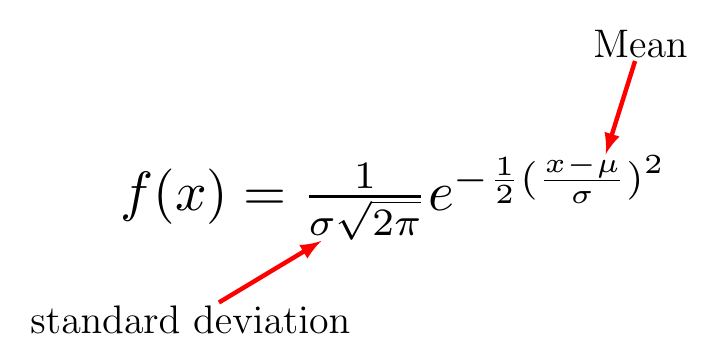
\begin{tikzpicture}
	\node[anchor=south east, inner sep=0] (eq) at (0, 0) {\scalebox{2}{$f(x) = \frac{1}{\sigma \sqrt{2 \pi}} e^{-{\frac{1}{2}} (\frac{x-\mu}{\sigma})^2}$}};
	\node[anchor=east, inner sep=1] (anot1) at (-4, -1) {\Large standard deviation};
	\node[anchor=west, inner sep=1] (anot2) at (-1, 2.5) {\Large Mean};
	\draw[-latex, ultra thick, red] (anot1) -- (eq);
	\draw[-latex, ultra thick, red] (anot2) -- (-0.8, 1.1) (eq); 
	\end{tikzpicture}
\end{frame}
%---------------------------------------------------------

%---------------------------------------------------------
%Example annotation
\begin{frame}
\frametitle{Sample Annotation}
\centering
	\begin{tikzpicture}
	\node [anchor=west] (note) at (-2,6) {\Large Gear Symbol};
	\node [anchor=west] (name) at (-2,4) {\Large Group Name};
	\begin{scope}[xshift=1cm]
	    \node[anchor=south west,inner sep=0] (image) at (0,0) {
\includegraphics[width=0.7\textwidth]{./logos/EnriqueGroupEh.png}};
	    \begin{scope}[x={(image.south east)},y={(image.north west)}]
		\draw[red,ultra thick,rounded corners] (0.38,0.80) rectangle (0.55,0.55);
		\draw[-latex, ultra thick, red, anchor=north] (note) to[out=0, in=-120] (0.48,0.55);
		    \draw[-stealth, line width=5pt, cyan] (name) -- ++(0.4, -0.0);
	    \end{scope}
	\end{scope}
	\end{tikzpicture}
\end{frame}
%---------------------------------------------------------

%---------------------------------------------------------
%Example of block flow chart
\begin{frame}
\frametitle{Sample Block Chart}
\centering
	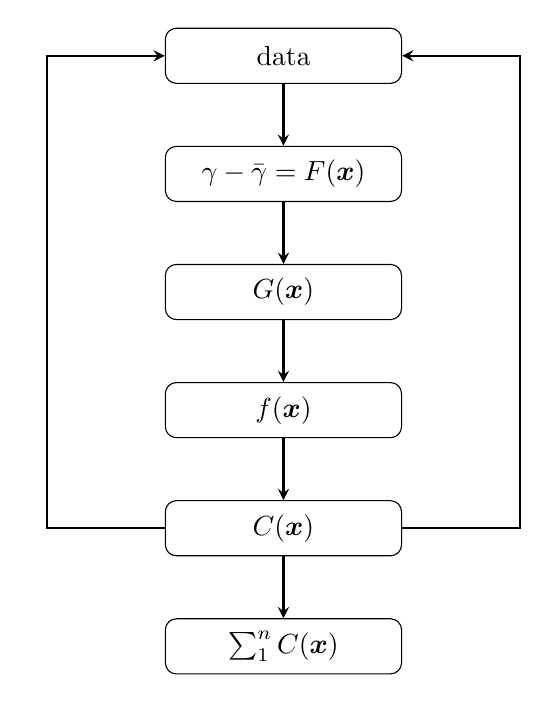
\begin{tikzpicture}[node distance=1.5cm]
		\node(b0) [block] {data};
		\node(b1) [block, below of=b0] {$\gamma - \bar\gamma = F(\bm{x})$};
		\node(b2) [block, below of=b1] {$G(\bm{x})$};
		\node(b3) [block, below of=b2] {$f(\bm{x})$};
		\node(b4) [block, below of=b3] {$C(\bm{x})$};
		\node(b5) [block, below of=b4] {$\sum_1^n C(\bm{x})$};
		\draw [arrow] (b0) -- (b1);
		\draw [arrow] (b1) -- (b2);
		\draw [arrow] (b2) -- (b3);
		\draw [arrow] (b3) -- (b4);
		\draw [arrow] (b4) -- +(-3,0) |- (b0) node[near start,sloped,above] {};
		\draw [arrow] (b4) -- +(+3,0) |- (b0) node[near start,sloped,above] {};
		\draw [arrow] (b4) -- (b5);
	\end{tikzpicture}
\end{frame}
%---------------------------------------------------------

%---------------------------------------------------------
% Example of logical flow chart
\begin{frame}
\frametitle{Sample Logical Flow Chart}

\begin{columns}

\column{0.5\textwidth}
\centering
	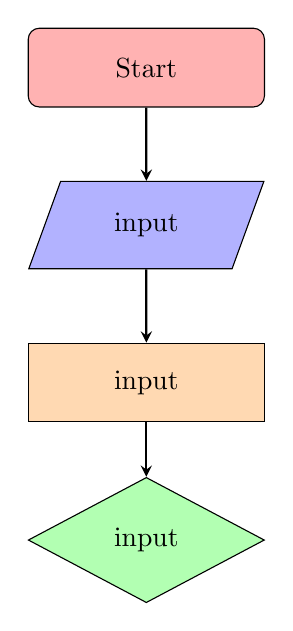
\begin{tikzpicture}[node distance=2cm]
		\node(start) [startstop] {Start};
		\node(in1) [io, below of=start] {input};
		\node(in2) [process, below of=in1] {input};
		\node(in3) [decision, below of=in2] {input};
		\draw [arrow] (start) -- (in1);
		\draw [arrow] (in1) -- (in2);
		\draw [arrow] (in2) -- (in3);
	\end{tikzpicture}

\column{0.5\textwidth}
	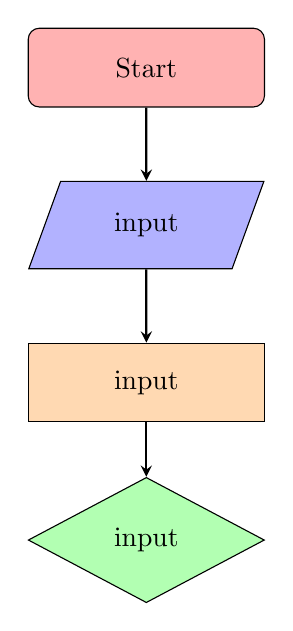
\begin{tikzpicture}[node distance=2cm]
		\node(start) [startstop] {Start};
		\node(in1) [io, below of=start] {input};
		\node(in2) [process, below of=in1] {input};
		\node(in3) [decision, below of=in2] {input};
		\draw [arrow] (start) -- (in1);
		\draw [arrow] (in1) -- (in2);
		\draw [arrow] (in2) -- (in3);
	\end{tikzpicture}
\end{columns}

\end{frame}
%---------------------------------------------------------

%---------------------------------------------------------
%Example of including figures
\begin{frame}
	\frametitle{Sample Include Figure}
	\begin{figure}[h]
		\centering
		%
\includegraphics[width=0.25\textwidth]{./logos/EnriqueGroupEh.png}
		\adjincludegraphics[,width=0.4\textwidth,trim={{.05\width} 0 {.0\width} 0},clip]{./logos/EnriqueGroupEh.png}

	\end{figure}
\end{frame}
%---------------------------------------------------------

%---------------------------------------------------------
%Changing visivility of the text
\begin{frame}
	\frametitle{Sample frame title}
	This is a text in second frame. For the sake of showing an example.

	\begin{itemize}
		\item<1-> Text visible on slide 1
		\item<2-> Text visible on slide 2
		\item<3> Text visible on slides 3
		\item<4-> Text visible on slide 4
	\end{itemize}
\end{frame}

%---------------------------------------------------------


%---------------------------------------------------------
%Example of the \pause command
\begin{frame}
	In this slide \pause

	the text will be partially visible \pause

	And finally everything will be there
\end{frame}
%---------------------------------------------------------

\section{Second section}

%---------------------------------------------------------
%Highlighting text
\begin{frame}
	\frametitle{Sample frame title}

	In this slide, some important text will be
	\alert{highlighted} because it's important.
	Please, don't abuse it.

	\begin{block}{Remark}
		Sample text
	\end{block}

	\begin{alertblock}{Important theorem}
		Sample text in red box
	\end{alertblock}

	\begin{examples}
		Sample text in green box. The title of the block is ``Examples".
	\end{examples}
\end{frame}
%---------------------------------------------------------


%---------------------------------------------------------
%Two columns
\begin{frame}
	\frametitle{Two-column slide}
	\begin{columns}
		\column{0.5\textwidth}
		This is a text in first column.
		$$E=mc^2$$
		\begin{itemize}
			\item First item
			\item Second item
		\end{itemize}

		\column{0.5\textwidth}
		This text will be in the second column
		and on a second tought this is a nice looking
		layout in some cases.
	\end{columns}
\end{frame}
%---------------------------------------------------------

\end{document}
